\documentclass[12pt,a4paper]{article}

% ----- GROUPED PACKAGES -----
% General Utilities
\usepackage[utf8]{inputenc}
\usepackage{geometry}
\usepackage{float}
\usepackage{afterpage}
\usepackage{enumitem}
\usepackage{ragged2e}
\usepackage[normalem]{ulem}

% Graphics and Drawing
\usepackage{graphicx}
\usepackage{pgf}
\usepackage{tikz}
\usepackage{svg}
\usepackage{stanli}
\usepackage{wrapfig}
\usepackage{rotating}
\usepackage[table]{xcolor}

% Math and Science
\usepackage{amsmath}
\usepackage{siunitx}

% Tables and Figures
\usepackage{booktabs}
\usepackage{caption}
\usepackage{subcaption}
\usepackage{multirow}

% Document Structure and Layout
\usepackage{titlesec}
\usepackage{titling}
\usepackage{pgfpages}
\usepackage{changepage}

% Code Listings
\usepackage{listings}

% Referencing
\usepackage[colorlinks=true, allcolors=blue]{hyperref}

% ----- CUSTOM DEFINITIONS -----

% Custom list settings
\setlist[itemize]{noitemsep, topsep=0pt, parsep=0pt, partopsep=0pt, leftmargin=*,
                 labelsep=0.5em, itemsep=1pt, label=\textbullet, font=\small}

% Custom section spacing
\titlespacing*{\section}{2pt}{*2}{*2}
\titlespacing*{\subsection}{3pt}{*3}{*3}

% Custom table row colors
\definecolor{tablerow1}{RGB}{240,240,240}
\definecolor{tablerow2}{RGB}{220,230,240}

% Enhanced VS Code Inspired with Light Background
\definecolor{vscode-blue}{RGB}{0,0,255}
\definecolor{vscode-green}{RGB}{0,128,0}
\definecolor{vscode-red}{RGB}{163,21,21}
\definecolor{vscode-purple}{RGB}{163,53,238}
\definecolor{vscode-orange}{RGB}{200,90,30}

\lstdefinestyle{vscodelight}{
    basicstyle=\ttfamily\footnotesize\bfseries\color[RGB]{30,30,30},
    backgroundcolor=\color[RGB]{240,248,255},
    rulecolor=\color[RGB]{200,200,200},
    frame=single,
    frameround=tttt,
    framesep=6pt,
    xleftmargin=13pt,
    xrightmargin=13pt,
    numbers=left,
    numberstyle=\tiny\bfseries\color[RGB]{100,100,100},
    numbersep=10pt,
    breaklines=true,
    breakatwhitespace=true,
    showstringspaces=false,
    tabsize=6,
    captionpos=b,
    keywordstyle=\bfseries\color{vscode-blue},
    commentstyle=\itshape\bfseries\color{vscode-green},
    stringstyle=\bfseries\color{vscode-red},
    identifierstyle=\bfseries\color[RGB]{30,30,30},
    emphstyle=\bfseries\color{vscode-purple},
    emph={function,class,return,import,from,as},
    % (removed moredelim=[is]{@}{@}: it would swallow NumPy's @ matrix-multiply operator)
    linewidth=\linewidth,
    xleftmargin=0pt,
    xrightmargin=0pt
}

\lstset{style=vscodelight}

% Additional formatting for academic papers
\lstset{
    aboveskip=0.7\baselineskip,
    belowskip=0.7\baselineskip,
    abovecaptionskip=5pt,
    belowcaptionskip=5pt,
    % captionmargin=5pt,  (not a listings key: breaks compilation once a listing is used)
    escapechar=!,
    prebreak=\raisebox{0ex}[0ex][0ex]{\ensuremath{\hookleftarrow}},
    postbreak=\raisebox{0ex}[0ex][0ex]{\ensuremath{\hookrightarrow}},
    extendedchars=true
}

% For even wider code blocks
\lstset{
    frame=lrtb,
    framerule=0.5pt,
    % framextendmargin=5pt (not a listings key)
}

% Set page margins
\geometry{a4paper, margin=1in}

% Figures live in report/figures (generated by experiments/), logos next to this file
\graphicspath{{../figures/}{./}}
\usepackage{amssymb}
\usetikzlibrary{positioning, arrows.meta, calc, angles, quotes}
\lstset{language=Python}
\newcommand{\T}{^{\mathsf{T}}}
\newcommand{\wrapop}{\operatorname{wrap}}

% Customize title style
\pretitle{\begin{center}\LARGE\bfseries}
\posttitle{\par\end{center}\vskip 0.3em}
\preauthor{\begin{center}\large}
\postauthor{\end{center}}
\predate{\begin{center}\large}
\postdate{\end{center}}


\begin{document}

% Title page
\begin{titlepage}
    \centering
    \vspace{1cm}

    
\includegraphics[width=0.25\linewidth]{university (1).png}\\
    \vspace{0.4cm}
    
\includegraphics[width=0.2\linewidth]{entc (2).png}\\
    
    \vspace{0.4cm}
    {\Large University of Moratuwa \par}
     \vspace{0.2cm}
     {\Large Department of Electronic and Telecommunication \par}

    \vspace{1cm}
    
    \rule{\textwidth}{0.4pt}
    \vspace{1cm}
    
    {\Large\bfseries Extended Kalman Filter for Human Joint-Angle Estimation from Monocular Video \par}
    \vspace{1cm}
    {\Large Mini Project: Implementing State Estimation Filters \par}
    {\Large EN4594 - Autonomous Systems \par}
    \vspace{2cm}
    \rule{\textwidth}{0.4pt}
    \begin{center}
    \vspace{0.2cm}
    \vspace{0.5cm}
    \textbf{\Large Sulojan.R - 220626V}\\

\end{center}
    
    \vfill

    \begin{center}
        {\Large 20th of Nov 2026}
    \end{center}
\end{titlepage}

% ============================================================================ ABSTRACT + TOC
\begin{abstract}
\noindent
State of the art deep pose estimation networks such as YOLO26-Pose give body keypoints for every video frame, but their output
jitters, drops out under occlusion, and lets the bones between keypoints change length from frame to
frame. This project builds an \textbf{Extended Kalman Filter (EKF)} that turns these noisy detections into
\textbf{smooth, physically consistent knee and hip angles}. The person is modelled as a planar stick
figure: a root position, nine absolute segment angles, their velocities and seven bone lengths (29 states).
The measurement model maps this state to 12 keypoints through nonlinear forward kinematics, and the filter
linearises it with an analytic Jacobian. Four additions make the filter robust on real detector output:
a confidence-adaptive measurement covariance with partial updates, a per-keypoint $\chi^2$ innovation
gate, joint-limit projection, and a track-loss re-initialisation that recovers a limb after long
occlusions. On a simulator with known ground truth the filter is statistically consistent
(NEES/dim $=1.03$, NIS/dof $=0.99$) and cuts the knee-angle error from $9.6^\circ$ to $5.1^\circ$.
On 37 side-view squat clips from Penn Action it reduces angle jitter by $4\times$, more than halves
bone-length variation, keeps an estimate in 99.9\% of frames, and adds only $\approx 0.5$\,ms per
frame, so a nano-sized detector with the EKF produces smoother angles than a $9\times$ larger
detector alone. Remaining failure modes are analysed and a concrete fix is proposed.
\end{abstract}

\vspace{1em}
\noindent\textbf{Source code:} \url{https://github.com/Sulojan2027/ekf-pose} (Python/NumPy).

\setcounter{tocdepth}{1}
\tableofcontents
\newpage

% ============================================================================ 1 INTRODUCTION
\section{Introduction}

Knee and hip angles during a squat are standard quantities in strength coaching and rehabilitation.
Measuring them normally needs markers, IMUs or a motion-capture lab. A phone camera with a pose
network is a cheap alternative: YOLO26-Pose \cite{ultralytics} returns 17 COCO keypoints
\cite{coco} per frame in about 6\,ms on a laptop GPU. The raw output has \textbf{three major problems} for joint-angle
measurement (Fig.~\ref{fig:overlay}):
\begin{itemize}
    \item \textbf{Jitter.} Each frame is detected independently, so angles computed from raw keypoints
          shake from frame to frame.
    \item \textbf{Dropouts and outliers.} Keypoints disappear or jump to the wrong limb under occlusion and
          motion blur, sometimes with high confidence.
    \item \textbf{No body model.} Nothing ties keypoints together, so the thigh, a rigid bone, appears to
          change length by 10\% or more between frames.
\end{itemize}

\paragraph{Why an EKF, and not a linear Kalman filter?}
A linear Kalman filter \cite{kalman} can only smooth each keypoint's $x$ and $y$ independently. It
cannot hold a bone at a constant length, cannot say that a knee does not bend past $165^\circ$, and never
estimates a joint angle itself. If instead the \emph{state} contains the segment angles and bone
lengths, all three come for free, but a keypoint's position then depends on the angles through
$\sin$ and $\cos$: the measurement model $h(\mathbf{x})$ is \emph{nonlinear}. The EKF
\cite{simon,barshalom} handles this by linearising $h$ around the current estimate with its Jacobian
$H$. The application is therefore \emph{target tracking of an articulated body}, and the filter is
an EKF.

\paragraph{Contributions.}
\begin{enumerate}[leftmargin=*, itemsep=1pt]
    \item A 29-dimensional planar skeleton state with \textbf{online bone-length self-calibration},
          its forward-kinematics measurement model and an analytic, unit-tested Jacobian.
    \item \textbf{Confidence-adaptive noise} $R$ with partial updates, and a
          \textbf{per-keypoint $\chi^2$ innovation gate} that rejects a single wrong keypoint without
          discarding the frame.
    \item \textbf{Joint-limit projection} and a \textbf{track-loss re-initialisation} rule that fixes a
          failure of the linearised gate after long occlusions (found in experiment E4).
    \item A complete evaluation: a simulator with known ground truth (accuracy, NEES/NIS consistency,
          occlusion), real-data comparison against two baselines on Penn Action \cite{penn}, an ablation of
          every component, and an edge-deployment study (YOLO26n vs YOLO26x).
    \item A dataset finding: Penn Action's left/right joint labels are mirrored relative to the COCO
          convention used by YOLO; correcting this lowers the ground-truth vs.\ detector error in all
          47 clips used.
\end{enumerate}

% ============================================================================ 2 METHODOLOGY
\section{Methodology}

\subsection{Conventions and state vector}

All quantities are in image coordinates (pixels), with $x$ to the right and $y$ \emph{down}.
A segment with absolute angle $\theta$ points along the unit vector
\begin{equation}
  \mathbf{u}(\theta) = \begin{bmatrix}\cos\theta\\ \sin\theta\end{bmatrix},\qquad
  \mathbf{u}_\perp(\theta) = \mathbf{u}(\theta + \tfrac{\pi}{2}) = \begin{bmatrix}-\sin\theta\\ \cos\theta\end{bmatrix}.
\end{equation}
Because $y$ points down, an upright torso has $\theta_t\approx-\pi/2$ and a hanging limb
$\theta\approx+\pi/2$. All angles are wrapped to $(-\pi,\pi]$.
The state (Fig.~\ref{fig:skeleton}) is
\begin{equation}
  \begin{split}
  \mathbf{x} = \big[\,&\underbrace{\mathbf{p}_0}_{2}\;\;
  \underbrace{\theta_t,\theta_{ua}^{L},\theta_{fa}^{L},\theta_{ua}^{R},\theta_{fa}^{R},
  \theta_{th}^{L},\theta_{sh}^{L},\theta_{th}^{R},\theta_{sh}^{R}}_{9\ \text{absolute angles}}\\
  &\underbrace{\dot{\mathbf{p}}_0,\ \dot{\boldsymbol\theta}}_{2+9}\;\;
  \underbrace{L_t, W_s, W_h, L_{ua}, L_{fa}, L_{th}, L_{sh}}_{7\ \text{lengths}}\big]\T\in\mathbb{R}^{29},
  \end{split}
\end{equation}
where $\mathbf{p}_0$ is the mid-hip (root), $W_s, W_h$ are the half shoulder and hip widths
(perpendicular to the torso), and left and right limbs share one length per segment type.
Joint angles are differences of absolute angles. The same definitions are used for the ground truth,
the baselines and the EKF:
\begin{equation}
  \text{knee} = \big|\wrapop(\theta_{th} - \theta_{sh})\big|,\qquad
  \text{hip}  = \pi - \big|\wrapop(\theta_{t} - \theta_{th})\big|,
  \label{eq:flexion}
\end{equation}
both $0^\circ$ when standing straight and independent of which way the person faces.

\begin{figure}[t]
\centering
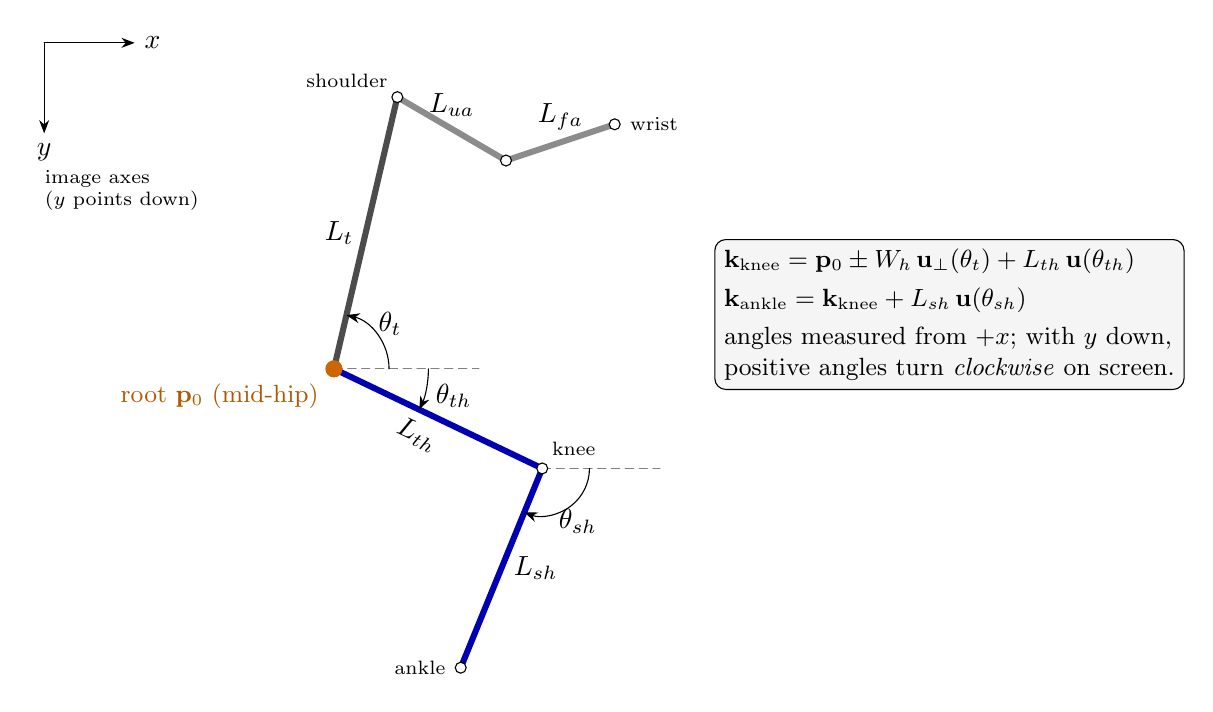
\begin{tikzpicture}[scale=1.15, >=Stealth, line cap=round,
    seg/.style={line width=2.2pt, blue!70!black}, jnt/.style={circle, fill=white, draw=black, inner sep=1.4pt}]
  % image axes
  \draw[->] (-3.2,3.6) -- (-2.2,3.6) node[right] {$x$};
  \draw[->] (-3.2,3.6) -- (-3.2,2.6) node[below] {$y$};
  \node[font=\scriptsize, align=left, anchor=north west] at (-3.3,2.3) {image axes\\($y$ points down)};
  \coordinate (P0) at (0,0); \coordinate (SH) at (0.7,3.0);
  \coordinate (KN) at (2.3,-1.1); \coordinate (AN) at (1.4,-3.3);
  \coordinate (EL) at (1.9,2.3); \coordinate (WR) at (3.1,2.7);
  \draw[seg, black!70] (P0) -- node[left, black] {$L_t$} (SH);
  \draw[seg] (P0) -- node[below, sloped, black, pos=0.45] {$L_{th}$} (KN);
  \draw[seg] (KN) -- node[right, black] {$L_{sh}$} (AN);
  \draw[seg, black!45] (SH) -- node[above, black] {$L_{ua}$} (EL);
  \draw[seg, black!45] (EL) -- node[above, black] {$L_{fa}$} (WR);
  % angle references (+x axis) and arcs
  \draw[densely dashed, gray] (P0) -- ++(1.6,0) coordinate (RX0);
  \draw[densely dashed, gray] (KN) -- ++(1.3,0) coordinate (RX1);
  \pic[draw, <-, "$\theta_{th}$", angle eccentricity=1.3, angle radius=1.2cm] {angle = KN--P0--RX0};
  \pic[draw, <-, "$\theta_{sh}$", angle eccentricity=1.35, angle radius=0.6cm] {angle = AN--KN--RX1};
  \pic[draw, ->, "$\theta_{t}$", angle eccentricity=1.3, angle radius=0.7cm] {angle = RX0--P0--SH};
  \foreach \p in {SH,KN,AN,EL,WR} \node[jnt] at (\p) {};
  \node[circle, fill=orange!80!black, inner sep=2.2pt] at (P0) {};
  \node[below left=2pt and 2pt, orange!70!black, font=\small] at (P0) {root $\mathbf{p}_0$ (mid-hip)};
  \node[above left, font=\scriptsize] at (SH) {shoulder};
  \node[above right=1pt and 0pt, font=\scriptsize] at (KN) {knee};
  \node[left=2pt, font=\scriptsize] at (AN) {ankle};
  \node[right=2pt, font=\scriptsize] at (WR) {wrist};
  % keypoint equation
  \node[draw, rounded corners, fill=gray!8, align=left, font=\small, anchor=west] at (4.2,0.6)
    {$\mathbf{k}_{\text{knee}} = \mathbf{p}_0 \pm W_h\,\mathbf{u}_\perp(\theta_t) + L_{th}\,\mathbf{u}(\theta_{th})$\\[3pt]
     $\mathbf{k}_{\text{ankle}} = \mathbf{k}_{\text{knee}} + L_{sh}\,\mathbf{u}(\theta_{sh})$\\[3pt]
     angles measured from $+x$; with $y$ down,\\positive angles turn \emph{clockwise} on screen.};
\end{tikzpicture}
\caption{Planar body model in image coordinates (side view, one side shown). Every keypoint is the root plus
a chain of segment vectors $\ell_i\,\mathbf{u}(\theta_i)$; lengths are states, so the filter calibrates
the person's bone lengths online.}
\label{fig:skeleton}
\end{figure}

\subsection{Process model: constant velocity with white-noise acceleration}

Between frames each position and angle keeps its velocity, and any change of velocity is random. For one
coordinate $q$ (a root coordinate or an angle) with velocity $\dot q$ and an acceleration $a_k$ that is
constant over the frame interval $\Delta t$:
\begin{align}
  \begin{bmatrix} q\\ \dot q\end{bmatrix}_{k+1} &=
  \underbrace{\begin{bmatrix}1 & \Delta t\\ 0 & 1\end{bmatrix}}_{F_{\text{blk}}}
  \begin{bmatrix} q\\ \dot q\end{bmatrix}_k +
  \underbrace{\begin{bmatrix}\Delta t^2/2\\ \Delta t\end{bmatrix}}_{\mathbf{g}} a_k,\qquad
  a_k\sim\mathcal{N}(0,\sigma^2),\\
  \Rightarrow\quad Q_{\text{blk}} &= \sigma^2\mathbf{g}\mathbf{g}\T =
  \sigma^2\begin{bmatrix}\Delta t^4/4 & \Delta t^3/2\\ \Delta t^3/2 & \Delta t^2\end{bmatrix}.
  \label{eq:Q}
\end{align}
$F\in\mathbb{R}^{29\times29}$ is the identity plus $\Delta t$ in the 11 position$\to$velocity couplings,
and $Q$ is block-diagonal with $\sigma=\sigma_a$ for the root, $\sigma=\sigma_{\ddot\theta}$ for the angles,
and a slow random walk $Q_{\ell\ell}=\sigma_L^2$ on the lengths. Penn Action gives no frame rate, so
$\Delta t = 1$ frame and the noise parameters are in px/frame$^2$ and rad/frame$^2$. The prediction is
linear and exact:
\begin{equation}
  \hat{\mathbf{x}}^- = F\hat{\mathbf{x}},\qquad P^- = FPF\T + Q.
\end{equation}

\subsection{Measurement model: forward kinematics}

The measurement is the 12 body keypoints of COCO (shoulders, elbows, wrists, hips, knees, ankles),
$\mathbf{z}\in\mathbb{R}^{24}$. Each keypoint is the root plus a sum of signed segment vectors along its
kinematic chain:
\begin{equation}
  \mathbf{k}_j(\mathbf{x}) = \mathbf{p}_0 + \sum_{i\in\mathcal{C}(j)} s_i\,\ell_i\,\mathbf{d}_i(\theta_{a_i}),
  \qquad \mathbf{d}_i\in\{\mathbf{u},\mathbf{u}_\perp\},\quad s_i=\pm1,
  \label{eq:fk}
\end{equation}
where $\mathcal{C}(j)$ is the list of segments from the root to keypoint $j$
(e.g.\ ankle: hip half-width, thigh, shank), $\ell_i$ the segment's length state and $a_i$ its angle
state. The sign $s_i$ is $+$ for left and $-$ for right on the width segments only. Angles enter through
$\cos$ and $\sin$ and multiply the lengths, so $h(\mathbf{x}) = [\mathbf{k}_1\T,\dots,\mathbf{k}_{12}\T]\T$
is nonlinear, which is what makes this an EKF problem.

\subsection{Analytic Jacobian}

One identity makes the derivation short: differentiating a direction vector rotates it by $+90^\circ$,
\begin{equation}
  \frac{d}{d\theta}\mathbf{u}(\theta) = \mathbf{u}_\perp(\theta),\qquad
  \frac{d}{d\theta}\mathbf{u}_\perp(\theta) = -\mathbf{u}(\theta).
\end{equation}
Differentiating (\ref{eq:fk}) term by term gives, for every segment $i$ on keypoint $j$'s chain,
\begin{equation}
  \frac{\partial\mathbf{k}_j}{\partial\mathbf{p}_0} = I_2,\qquad
  \frac{\partial\mathbf{k}_j}{\partial\theta_{a_i}} \mathrel{+}= s_i\,\ell_i\,\frac{d\mathbf{d}_i}{d\theta},\qquad
  \frac{\partial\mathbf{k}_j}{\partial\ell_i} \mathrel{+}= s_i\,\mathbf{d}_i,\qquad
  \frac{\partial\mathbf{k}_j}{\partial(\text{velocities})} = 0 .
\end{equation}
The ``$+=$'' matters: $\theta_t$ appears twice in each shoulder chain (torso along $\mathbf{u}$, half-width
along $\mathbf{u}_\perp$), so
$\partial\mathbf{k}_{\text{sh},L}/\partial\theta_t = L_t\,\mathbf{u}_\perp(\theta_t) - W_s\,\mathbf{u}(\theta_t)$.
$H\in\mathbb{R}^{24\times29}$ is sparse: a keypoint depends only on the root and on the angles and lengths of
its own chain.

\subsection{EKF update with adaptive noise, partial updates and gating}
\label{sec:update}

Every frame runs the loop in Fig.~\ref{fig:loop}. The three robustness steps all decide \emph{which rows}
of $\mathbf{z}$, $h$, $H$ and $R$ take part in the update, so they share one code path.

\begin{figure}[t]
\centering
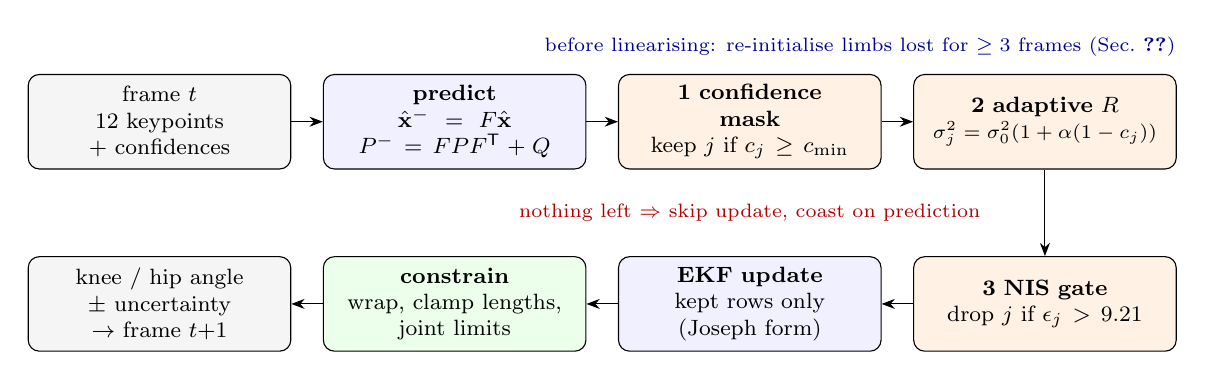
\begin{tikzpicture}[node distance=4mm and 4mm, >=Stealth, font=\footnotesize,
    box/.style={draw, rounded corners, align=center, minimum height=12mm, text width=31mm, fill=#1},
    box/.default=blue!6]
  \node[box=gray!8] (in) {frame $t$\\12 keypoints\\+ confidences};
  \node[box, right=of in] (pred) {\textbf{predict}\\$\hat{\mathbf{x}}^-=F\hat{\mathbf{x}}$\\$P^-=FPF\T+Q$};
  \node[box=orange!10, right=of pred] (mask) {\textbf{1 confidence}\\\textbf{mask}\\keep $j$ if $c_j\ge c_{\min}$};
  \node[box=orange!10, right=of mask] (R) {\textbf{2 adaptive $R$}\\\mbox{\scriptsize $\sigma_j^2=\sigma_0^2(1+\alpha(1-c_j))$}};
  \node[box=orange!10, below=11mm of R] (gate) {\textbf{3 NIS gate}\\drop $j$ if $\epsilon_j>9.21$};
  \node[box, left=of gate] (upd) {\textbf{EKF update}\\kept rows only\\(Joseph form)};
  \node[box=green!8, left=of upd] (con) {\textbf{constrain}\\wrap, clamp lengths,\\joint limits};
  \node[box=gray!8, left=of con] (out) {knee / hip angle\\$\pm$ uncertainty\\$\to$ frame $t{+}1$};
  \draw[->] (in) -- (pred); \draw[->] (pred) -- (mask); \draw[->] (mask) -- (R);
  \draw[->] (R) -- (gate); \draw[->] (gate) -- (upd); \draw[->] (upd) -- (con); \draw[->] (con) -- (out);
  \node[font=\scriptsize, text=red!70!black, align=center] at ($(mask.south)!0.5!(upd.north)$)
     {nothing left $\Rightarrow$ skip update, coast on prediction};
  \node[font=\scriptsize, text=blue!60!black, align=center, above=1mm of mask, xshift=14mm]
     {before linearising: re-initialise limbs lost for $\ge 3$ frames (Sec.~\ref{sec:reinit})};
\end{tikzpicture}
\caption{One EKF frame. Steps 1--3 (orange) choose which keypoint rows enter the update; if none survive,
the filter coasts on the prediction and its uncertainty grows.}
\label{fig:loop}
\end{figure}

\paragraph{1. Confidence mask (partial update).} Keypoints with confidence $c_j < c_{\min}=0.3$ are
removed. If YOLO detects no person, all confidences are 0 and the filter simply predicts.

\paragraph{2. Confidence-adaptive $R$.} A less confident keypoint should move the state less:
\begin{equation}
  \sigma_j = \sigma_0\sqrt{1+\alpha\,(1-c_j)},\qquad
  R = \operatorname{diag}(\sigma_{j_1}^2,\sigma_{j_1}^2,\dots,\sigma_{j_k}^2,\sigma_{j_k}^2),
\end{equation}
for the $k$ kept keypoints ($x$ and $y$ of a keypoint share $\sigma_j$).

\paragraph{3. Per-keypoint NIS gate.} For each kept keypoint $j$ with rows $r_j=\{2j,2j{+}1\}$,
\begin{equation}
  \mathbf{y}_j = \mathbf{z}_j - \mathbf{k}_j(\hat{\mathbf{x}}^-),\qquad
  S_{jj} = H_{r_j}P^-H_{r_j}\T + \sigma_j^2 I_2,\qquad
  \epsilon_j = \mathbf{y}_j\T S_{jj}^{-1}\mathbf{y}_j .
\end{equation}
If the model is right, $\epsilon_j\sim\chi^2_2$, so a keypoint with $\epsilon_j > \chi^2_2(0.99) = 9.21$
is too surprising and is dropped for this frame. Using the $2\times2$ diagonal block rather than the full
$S$ asks ``is \emph{this} keypoint plausible on its own?'', so one bad keypoint cannot hide among good ones.

\paragraph{Update.} With $\mathbf{z}$, $h$, $H$, $R$ restricted to the kept rows:
\begin{align}
  \mathbf{y} &= \mathbf{z} - h(\hat{\mathbf{x}}^-), & S &= HP^-H\T + R, & K &= P^-H\T S^{-1},\\
  \hat{\mathbf{x}} &= \hat{\mathbf{x}}^- + K\mathbf{y}, & P &= (I-KH)\,P^-(I-KH)\T + KRK\T .
\end{align}
The \textbf{Joseph form} of the covariance update is valid for any gain and keeps $P$ symmetric positive
semi-definite despite rounding; $K$ is computed with a linear solve, never an explicit inverse. The full
normalised innovation $\mathbf{y}\T S^{-1}\mathbf{y}$ and its degrees of freedom ($2k$) are logged for the
consistency checks.

\subsection{Constraints}

After every update the angles are wrapped, $P$ is symmetrised, lengths are clamped (widths
$\ge 1$\,px, which allows a side view where the shoulders overlap; other lengths $\ge 5$\,px), and
\textbf{joint limits} are applied by projection: if $|\wrapop(\theta_{th}-\theta_{sh})| > 165^\circ$
the shank angle is moved back onto the limit (elbows: $160^\circ$). The projection is sign-agnostic, so
left- and right-facing clips both work. Projecting the mean while leaving $P$ unchanged is the simplest
member of the constrained-Kalman-filter family \cite{simon_constraints}; estimate projection and
truncated-Gaussian methods also update $P$.

\subsection{Initialisation by inverse kinematics}

The filter starts at the first frame with at least one confident hip and shoulder. The forward kinematics
is inverted geometrically: root = mean of the hips; torso angle and length from mid-hip to mid-shoulder;
half-widths from the projection of each side onto $\mathbf{u}_\perp(\theta_t)$; limb angles
$\theta=\operatorname{atan2}(\Delta y,\Delta x)$ and lengths from the visible segments (mean of left and
right). Missing pieces fall back to the other side, then to anthropometric ratios of the torso length
\cite{winter}. Velocities start at 0, and $P_0$ is diagonal (10\,px, 0.2\,rad, 10\,px/frame, 0.3\,rad/frame,
5\,px). No update is done on the initialisation frame.

\subsection{Track-loss recovery}
\label{sec:reinit}

Experiment E4 exposed a failure of the linearised filter. During a long occlusion the angle variance grows
until the true uncertainty is a curved ``banana'' that a Gaussian over angles cannot represent. When the
limb reappears, its keypoints are far from the prediction in the linearised metric, fail the gate on every
frame, and the limb is never re-acquired. The fix: a counter $n_j$ records how many consecutive frames
confident keypoint $j$ was gated. If both ends of a limb segment $(i,k)$ are confident and
$\max(n_i,n_k)\ge 3$, the segment angle is re-initialised from the measurement,
$\theta_a\leftarrow\operatorname{atan2}(\mathbf{k}_k-\mathbf{k}_i)$, its velocity is set to 0, and the rows
and columns of $a$ and its velocity in $P$ are zeroed before the initial variances are restored on the
diagonal (in the other order $P$ becomes singular). Zeroing the cross-covariances states that the new angle
is independent of the old belief.

% ============================================================================ 3 IMPLEMENTATION
\section{Implementation}

\subsection{Pipeline, data and environment}

Everything is implemented in Python 3.11 with NumPy and SciPy. Ultralytics \cite{ultralytics} is used
\emph{only} for \texttt{model.predict()}; the filter, baselines, simulator and metrics are our own code.
Experiments ran on a laptop (Intel i5-12450H, NVIDIA RTX 2050).

\paragraph{Dataset.} Penn Action \cite{penn} has 2{,}326 clips with 13 hand-annotated joints per frame and a
per-joint visibility flag; its joints 1--12 are exactly COCO keypoints 5--16. We keep squats seen from the
side (180 clips) in which one complete leg chain (shoulder, hip, knee, ankle) is visible in at least 80\% of
frames: 37 clips of Penn's test split are the \textbf{test set} and 10 clips of the train split are the
\textbf{tuning set}. All parameters are chosen on the tuning set only. Clips have 64--163 frames of
about $315\times480$\,px. Angles are scored only on frames where all of their joints are visible in the
ground truth, on the near-side leg.

\paragraph{Pose detection.} Each frame of the 47 clips is processed once by YOLO26n-pose and
YOLO26x-pose; for every frame the person with the largest box is kept and the keypoints, confidences and
inference times are cached, so every method sees identical input.

\paragraph{Left/right mirror fix.} While validating the data we found that Penn Action labels the
person's left and right in the opposite sense to COCO/YOLO in side views. Swapping Penn's L/R joint labels
lowered the ground-truth vs.\ YOLO keypoint error in \textbf{47 of 47} clips (median $\approx4\times$).
The loader applies the swap once, so that ``left knee'' means the same physical joint for the ground truth,
YOLO and the EKF; without it every angle error in Section~\ref{sec:results} would be inflated.

\subsection{Key code}

The table-driven measurement model makes the whole body cost no more code than one leg. Each chain entry is
\texttt{(angle index, length index, sign, perpendicular?)}, and $h$ and $H$ loop over the same table:
\begin{lstlisting}[caption={Forward kinematics $h(\mathbf{x})$ and analytic Jacobian $H$ (\texttt{ekf/skeleton.py}).}, label=lst:fk, basicstyle={\ttfamily\scriptsize\bfseries\color[RGB]{30,30,30}}]
def fk(x):
    z = np.zeros(N_Z)
    for j in range(N_KP):
        pos = x[P0].copy()
        for (a, l, s, perp) in CHAINS[j]:
            pos += s * x[l] * seg_dir(x[a], perp)[0]     # s * l * d(theta)
        z[2 * j: 2 * j + 2] = pos
    return z

def jacobian(x):
    H = np.zeros((N_Z, N_X))
    for j in range(N_KP):
        r = slice(2 * j, 2 * j + 2)
        H[r, P0] = np.eye(2)                             # dk/dp0 = I
        for (a, l, s, perp) in CHAINS[j]:
            d, dd = seg_dir(x[a], perp)                  # d and dd/dtheta
            H[r, a] += s * x[l] * dd                     # +=: theta_t is used twice
            H[r, l] += s * d
    return H
\end{lstlisting}

\begin{lstlisting}[caption={Measurement update on the rows that survived masking and gating (\texttt{ekf/ekf.py}).}, label=lst:update, basicstyle={\ttfamily\scriptsize\bfseries\color[RGB]{30,30,30}}]
rows = kept_rows(mask)                     # keypoint j -> rows 2j, 2j+1
z  = kp.reshape(-1)[rows]
y  = z - z_pred[rows]                      # innovation
Hk = H[rows]
R  = make_R(sigma, mask)                   # confidence-adaptive, diagonal
S  = Hk @ self.P @ Hk.T + R
K  = np.linalg.solve(S, Hk @ self.P).T     # K = P H^T S^-1 without an inverse
self.x = self.x + K @ y
A  = np.eye(sk.N_X) - K @ Hk
self.P = A @ self.P @ A.T + K @ R @ K.T    # Joseph form
\end{lstlisting}

\begin{lstlisting}[caption={Track-loss recovery for one limb segment $(a, i, k)$ (\texttt{ekf/ekf.py}).}, label=lst:reinit, basicstyle={\ttfamily\scriptsize\bfseries\color[RGB]{30,30,30}}]
usable = mask[i] and mask[k]
lost = max(self.n_rej[i], self.n_rej[k]) >= self.p.reinit_after
if usable and lost:
    v = a + sk.VEL_OFFSET
    self.x[a] = sk.seg_angle(kp[i], kp[k])     # trust the measurement
    self.x[v] = 0.0
    for idx in (a, v):                         # forget correlations first ...
        self.P[idx, :] = 0.0
        self.P[:, idx] = 0.0
    self.P[a, a] = sk.P0_STD_ANG ** 2          # ... then restore the variances
    self.P[v, v] = sk.P0_STD_VANG ** 2
\end{lstlisting}

\subsection{Verification}

The code has 45 unit tests. 26 test the skeleton: the analytic Jacobian is compared with central finite
differences, $H_{:,k}\approx[h(\mathbf{x}+\varepsilon\mathbf{e}_k)-h(\mathbf{x}-\varepsilon\mathbf{e}_k)]/2\varepsilon$
with $\varepsilon=10^{-6}$, on 20 random states (relative tolerance $10^{-5}$); a standing pose must have
shoulder $<$ hip $<$ knee $<$ ankle in $y$; velocity columns of $H$ are zero; and initialising from keypoints
generated by a known state must reproduce those keypoints ($h(\mathbf{x}_0)$ inverts the inverse kinematics).
8 test the filter: the structure of $F$, $Q$ symmetric PSD, adaptive $R$, lower knee error than raw
keypoints on a synthetic squat, convergence of the length states, NIS consistency when $R$ matches the
noise, coasting through a dropout, and gating of an outlier. The remaining 11 are known-answer tests of every metric, baseline and of the
simulator's noise model.

\subsection{Baselines and metrics}

Two baselines receive the same cached keypoints and the same threshold $c_{\min}$:
a \textbf{causal moving average} of each keypoint over the last $w$ frames, and a \textbf{per-keypoint
linear Kalman filter} (12 independent constant-velocity filters on $[x,y,\dot x,\dot y]$ with the same
adaptive $R$; no bones). For every method, knee and hip angles are computed from its keypoints with
(\ref{eq:flexion}) (for the EKF, from $h(\hat{\mathbf{x}})$). Metrics: angle RMSE vs.\ ground truth on
frames where all compared methods have an estimate (reported as the median over clips, robust to a few
failed clips), \textbf{jitter} = mean $|$second difference$|$ of the angle (deg/frame$^2$),
\textbf{lag} = shift maximising the cross-correlation with the ground truth, keypoint RMSE in \% of the
person's box height, \textbf{bone-length CV} (std/mean of thigh and shank length, \%), coverage, and
runtime. In simulation the full state is known, so filter consistency is checked with the normalised
estimation error squared (NEES) $\mathbf{e}\T P^{-1}\mathbf{e}$, $\mathbf{e}=\hat{\mathbf{x}}-\mathbf{x}$,
and the NIS.

\subsection{Simulator}

Synthetic side-view squats with random body size, depth and facing direction are generated in the same
29-D state space (the ankle is fixed on the floor and the root solved from it). A synthetic detector draws a
confidence $c_j\sim\text{Beta}(8,1.5)$ per keypoint, adds Gaussian noise with
$\sigma_j=3\sqrt{1+4(1-c_j)}$\,px to $h(\mathbf{x})$, and can add dropouts, occlusion windows and confident
outliers (40\,px jumps with $c\ge0.8$). The simulated noise has the same form as the adaptive $R$, so the
simulation is a best case for that component; the real-data ablation is the honest test.

% ============================================================================ 4 RESULTS
\section{Results}
\label{sec:results}

\subsection{Simulation (known ground truth)}

\paragraph{E1: tracking a squat.} Fig.~\ref{fig:e1} shows one synthetic squat. The EKF follows the true
knee angle with RMSE $4.7^\circ$ (raw keypoints: $8.1^\circ$) and the hip with $2.8^\circ$ (raw $6.8^\circ$),
and the truth lies inside the $\pm2\sigma$ band in 99\% of frames.

\begin{figure}[t]
\centering
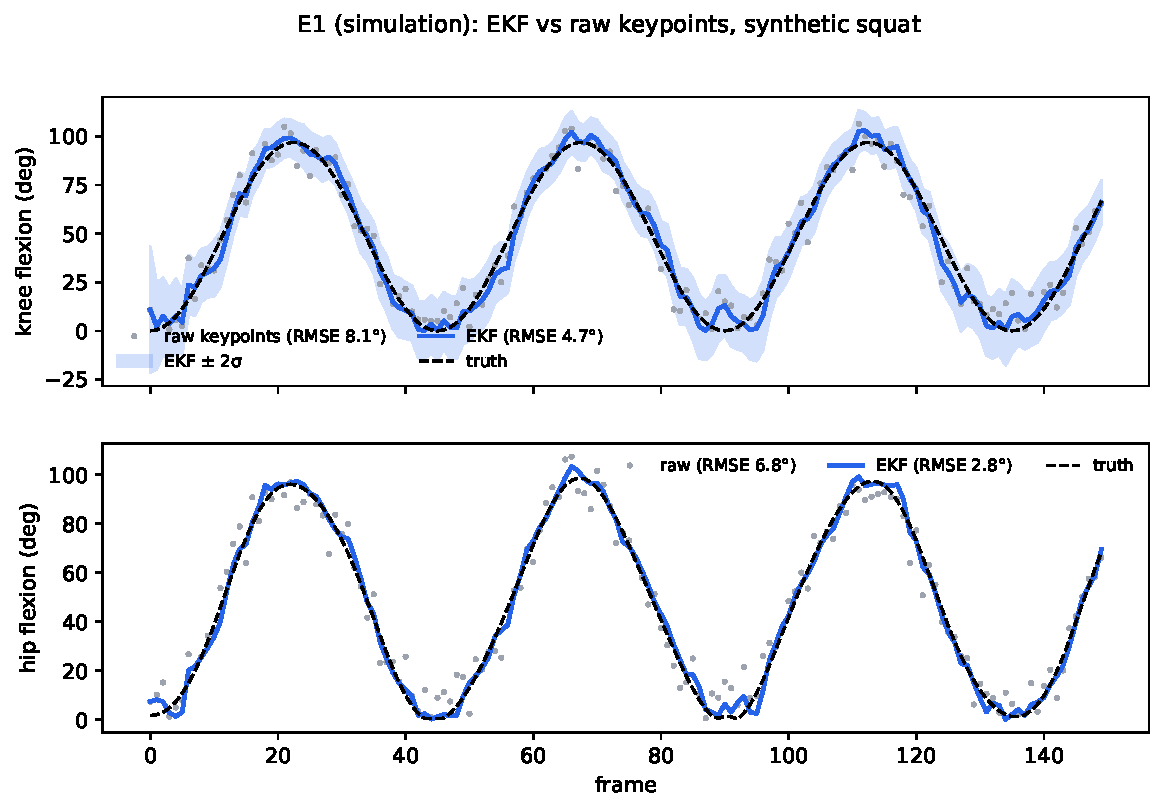
\includegraphics[width=0.86\linewidth]{e1_sim_angles.pdf}
\caption{E1 (simulation): knee (top) and hip (bottom) flexion. Grey dots: angles from raw noisy keypoints;
blue: EKF with its $\pm2\sigma$ band; dashed: truth. The band is wide at start-up and in the standing phase,
where the knee angle is least observable.}
\label{fig:e1}
\end{figure}

\paragraph{E2: process vs.\ measurement noise.} Fig.~\ref{fig:e2sim} sweeps the angular acceleration noise
$\sigma_{\ddot\theta}$ against $\sigma_0$ (10 seeds each). Trusting the motion model (small
$\sigma_{\ddot\theta}$, large $\sigma_0$) gives the smoothest angles (jitter 2.42) but lags and cuts the
bottom of the squat (RMSE $11.2^\circ$); trusting the detector gives low lag but high jitter (7.93). The
RMSE optimum ($4.33^\circ$) lies at the true noise level $\sigma_0\approx4$ and the middle
$\sigma_{\ddot\theta}=0.03$.

\begin{figure}[t]
\centering
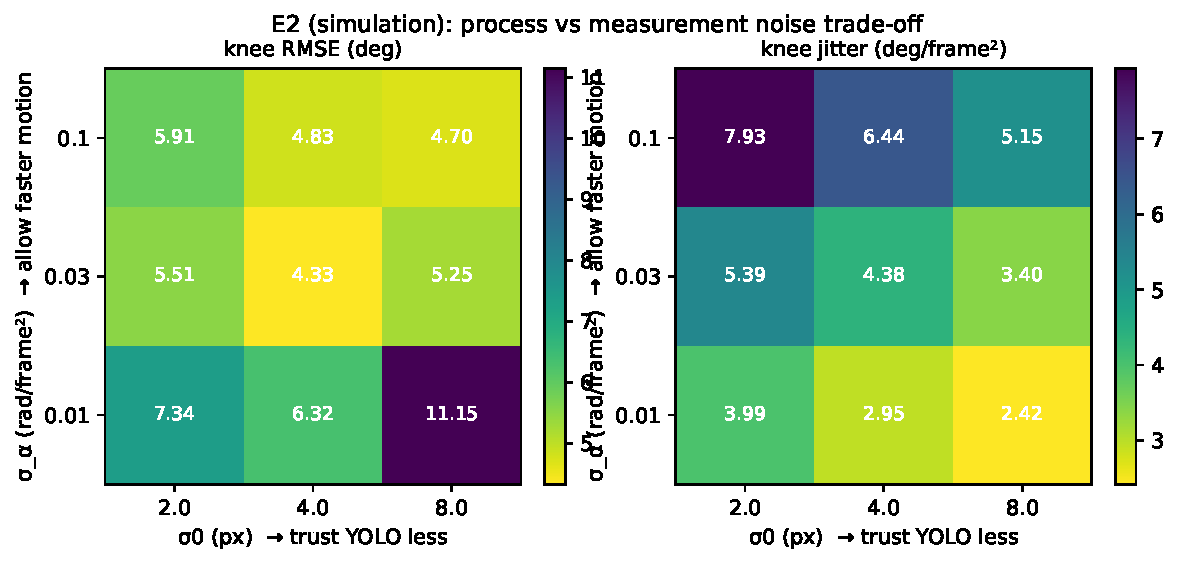
\includegraphics[width=0.82\linewidth]{e2_sim_sweep.pdf}
\caption{E2 (simulation): knee RMSE (left) and jitter (right) over a $3\times3$ grid of process noise
$\sigma_{\ddot\theta}$ (rows) and measurement noise $\sigma_0$ (columns). Accuracy and smoothness pull in
different directions.}
\label{fig:e2sim}
\end{figure}

\paragraph{E3: is the uncertainty honest?} If $P$ is correct, the NEES of a consistent filter follows
$\chi^2_{29}$ and the NIS $\chi^2_{\text{dof}}$. The average of $N$ independent runs then satisfies
$N\bar\epsilon\sim\chi^2_{N n}$, which gives the 95\% band in Fig.~\ref{fig:e3}. With truth generated
\emph{from} the filter's own model (``matched''), both statistics sit on 1 (Table~\ref{tab:e3}) and inside the
band in 93--94\% of frames, as expected for a 95\% band: the implementation of $F$, $Q$, $h$, $H$ and the
update is consistent. On the squat motion with default $Q$, $R$ the normalised values are about 0.5:
the filter is \emph{conservative}, i.e.\ its reported uncertainty is larger than its actual error.

\begin{figure}[t]
\centering
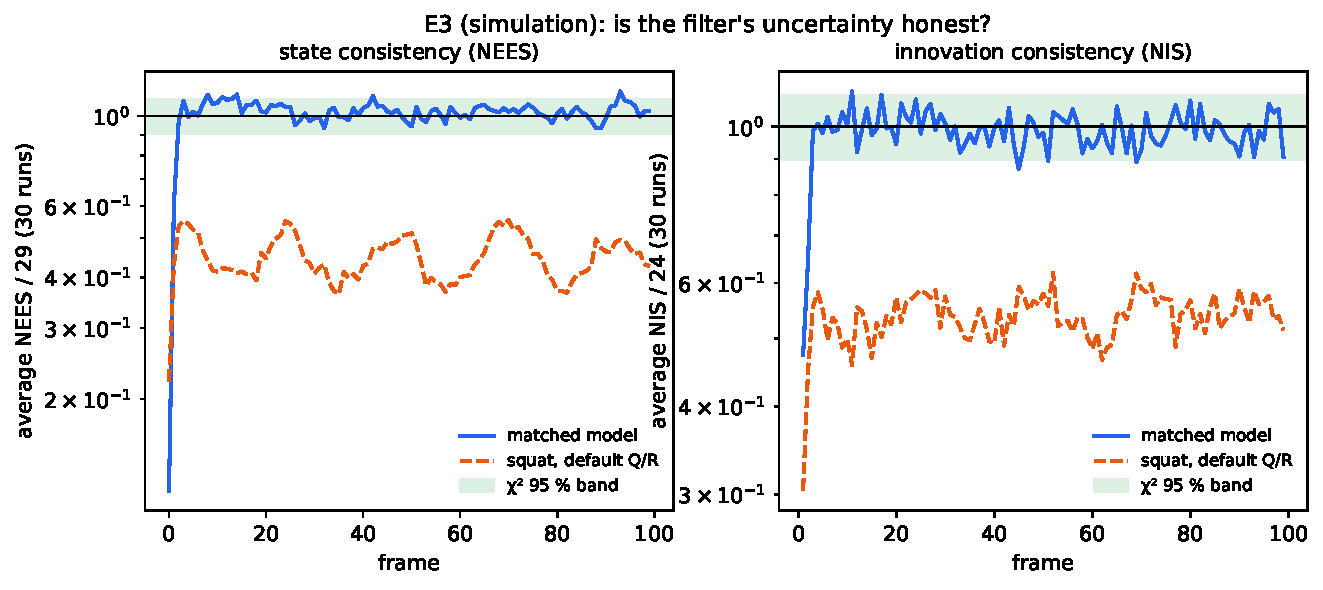
\includegraphics[width=0.88\linewidth]{e3_consistency.pdf}
\caption{E3 (simulation, 30 Monte-Carlo runs): average NEES/29 (left) and NIS/dof (right) against the
$\chi^2$ 95\% band (green). Blue: truth from the filter's own model; orange: squat motion (model mismatch).}
\label{fig:e3}
\end{figure}

\begin{table}[t]
\centering\small
\caption{E3: filter consistency, 30 Monte-Carlo runs (ideal: 1.00 and $\approx95\%$).}
\label{tab:e3}
\begin{tabular}{lcccc}
\toprule
Scenario & NEES/dim & NIS/dof & \% NEES in band & \% NIS in band\\
\midrule
Matched model & 1.03 & 0.99 & 93.3 & 94.4\\
Squat, default $Q$/$R$               & 0.45 & 0.54 & 0.0  & 0.0\\
\bottomrule
\end{tabular}
\end{table}

\paragraph{E4: occlusion and recovery.} Knees and ankles are hidden for 10, 20 or 30 frames
(Fig.~\ref{fig:e4}, Table~\ref{tab:e4}). During the gap the EKF coasts and its $2\sigma$ grows from
$10^\circ$ to $115$--$505^\circ$, correctly reporting that it no longer knows the knee angle. Without
re-initialisation the returning keypoints are gated as outliers and the error stays high ($114^\circ$
20 frames after a 20-frame gap). With track-loss recovery the knee is re-acquired within a few frames
(error $4.6^\circ$/$22.8^\circ$/$26.2^\circ$ averaged over the 20 frames after the gap).

\begin{figure}[t]
\centering
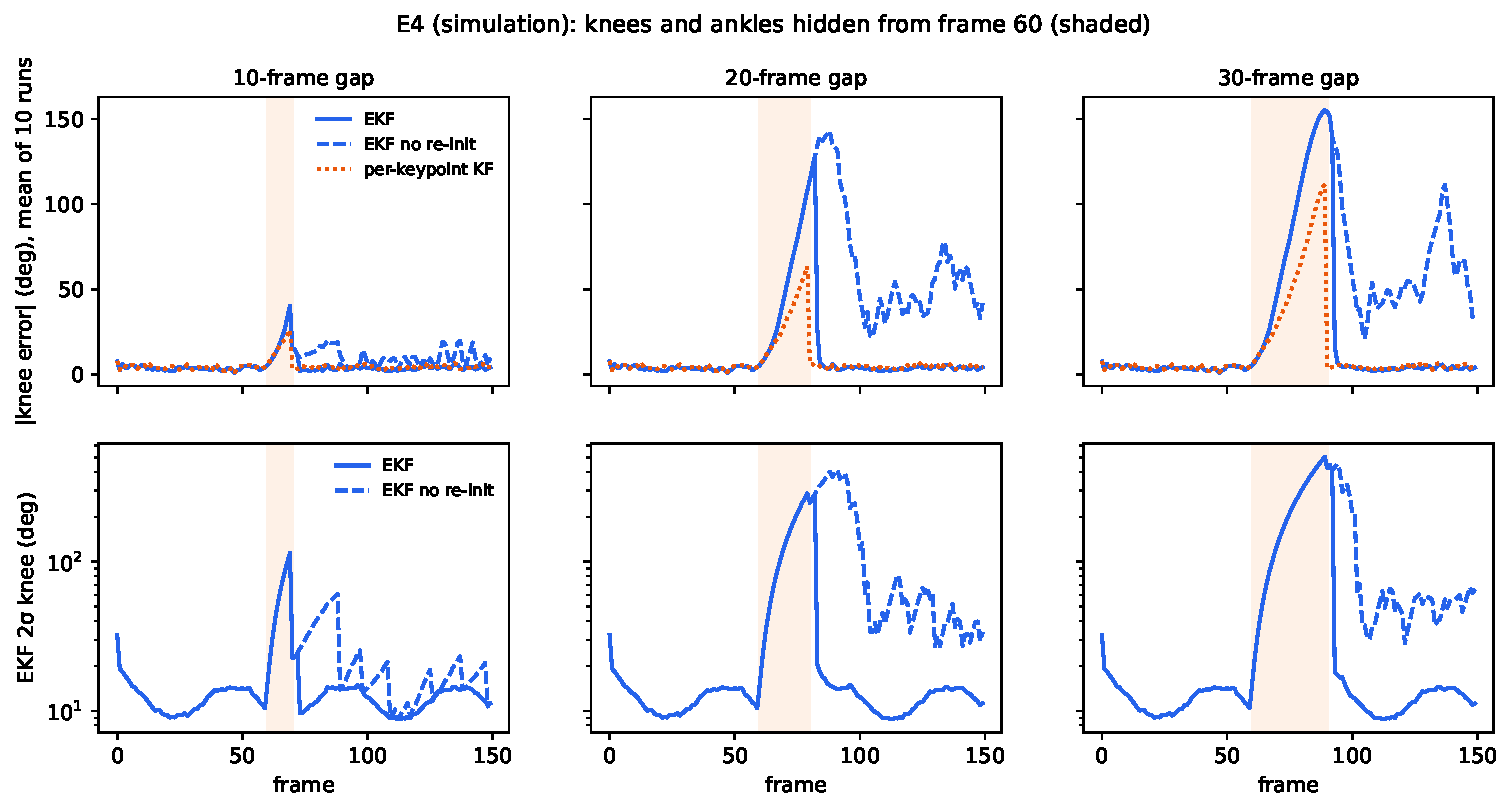
\includegraphics[width=\linewidth]{e4_occlusion.pdf}
\caption{E4 (simulation, mean of 10 runs): knee error (top) and the EKF's $2\sigma$ (bottom, log scale)
when knees and ankles are hidden from frame 60 (shaded). Dashed: without re-initialisation the
filter does not recover; solid: with it, the error drops back as soon as the keypoints return.}
\label{fig:e4}
\end{figure}

\begin{table}[t]
\centering\small
\caption{E4: mean knee error ($^\circ$) during the gap and over the 20 frames after it.}
\label{tab:e4}
\resizebox{\linewidth}{!}{%
\begin{tabular}{ccccccc}
\toprule
& \multicolumn{2}{c}{During gap} & \multicolumn{3}{c}{20 frames after gap} & EKF $2\sigma$\\
\cmidrule(lr){2-3}\cmidrule(lr){4-6}
Gap & EKF & per-kp KF & EKF & EKF no re-init & per-kp KF & at gap end\\
\midrule
10 & 19.0 & 15.7 & 4.6  & 14.7  & 4.1 & 115\\
20 & 48.2 & 30.6 & 22.8 & 114.4 & 4.7 & 287\\
30 & 78.5 & 51.0 & 26.2 & 78.0  & 4.4 & 505\\
\bottomrule
\end{tabular}}
\end{table}

\paragraph{E5 (simulation): ablation.} On a ``realistic'' scenario (lower confidences, 5\% missed
keypoints, 4\% confident 40\,px outliers; 20 seeds), the full EKF has the lowest error of all methods
(Table~\ref{tab:e5sim}): $5.1^\circ$ knee vs.\ $7.0^\circ$ for the per-keypoint KF and $9.6^\circ$ raw.
Removing adaptive $R$ or gating each costs accuracy, and removing both costs most.

\begin{table}[t]
\centering\small
\caption{E5 (simulation, 20 seeds): ablation on the realistic scenario.}
\label{tab:e5sim}
\begin{tabular}{lccc}
\toprule
Method & Knee RMSE ($^\circ$) & Hip RMSE ($^\circ$) & Knee jitter\\
\midrule
Raw keypoints              & 9.58 & 8.06 & 17.13\\
Moving average             & 10.17 & 10.00 & 3.47\\
Per-keypoint KF            & 7.03 & 5.75 & 7.21\\
\textbf{EKF (full)}        & \textbf{5.10} & \textbf{3.63} & 4.74\\
EKF, fixed $R$             & 5.43 & 3.82 & 5.45\\
EKF, no gating             & 5.62 & 3.90 & 5.09\\
EKF, fixed $R$ + no gating & 5.90 & 4.00 & 5.93\\
\bottomrule
\end{tabular}
\end{table}

\subsection{Real data (Penn Action, 37 test clips)}

\paragraph{Tuning.} $\sigma_{\ddot\theta}$ and $\sigma_0$ were grid-searched on the 10 tuning clips
(Fig.~\ref{fig:e2real}), minimising the median over clips of the mean knee/hip RMSE. The optimum is
$\sigma_{\ddot\theta}=0.02$\,rad/frame$^2$ and $\sigma_0=16$\,px, larger than the $\approx12$\,px typical
YOLO26n keypoint error (Section~\ref{sec:discussion}). The moving-average window ($w=7$) and the
per-keypoint KF's acceleration noise ($0.5$\,px/frame$^2$) were tuned the same way.

\begin{figure}[t]
\centering
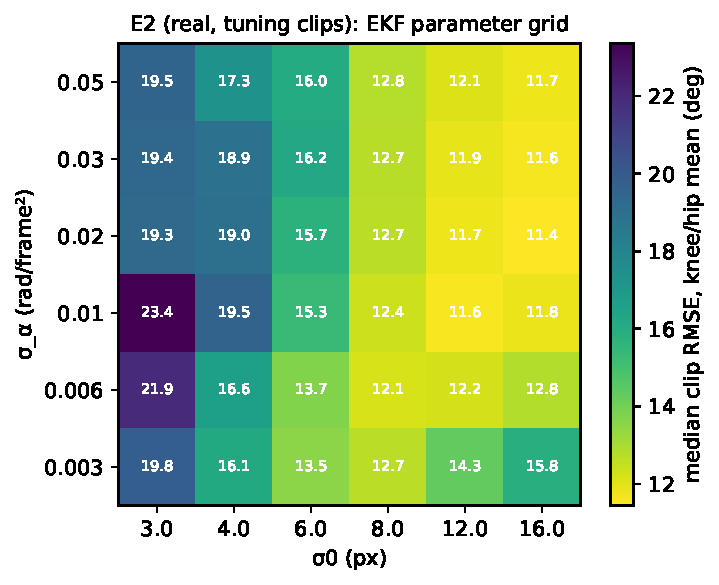
\includegraphics[width=0.5\linewidth]{e2_real_tune.pdf}
\caption{E2 (real, tuning clips only): median clip RMSE over the EKF parameter grid.}
\label{fig:e2real}
\end{figure}

\paragraph{E6: comparison of methods.} Table~\ref{tab:e6} and Fig.~\ref{fig:e6} compare all methods on
the test set. The EKF gives the smoothest angles among methods with a body-level output (knee jitter 1.30
vs.\ 5.41 raw), the most rigid bones (CV 4.8\% vs.\ 11.1\%), near-complete coverage (99.9\%), negligible
lag (0.24 frames) and a calibrated uncertainty band, at 0.6\,ms per frame. Its angle RMSE is higher than
raw YOLO; the cause is analysed in Section~\ref{sec:limits}, where the last row of the table is also
explained.

\begin{table}[t]
\centering\small
\caption{E6: methods on the 37 test clips (YOLO26n keypoints). RMSE: median over clips; other columns:
mean over clips. Ground-truth labels themselves have jitter 2.36 and bone CV 9.31\%.}
\label{tab:e6}
\setlength{\tabcolsep}{4pt}
\resizebox{\linewidth}{!}{%
\begin{tabular}{lccccccc}
\toprule
Method & Knee & Hip & Knee & Bone & Lag & Coverage & Time\\
       & RMSE ($^\circ$) & RMSE ($^\circ$) & jitter & CV (\%) & (frames) & (\%) & (ms)\\
\midrule
Raw YOLO26n              & 9.60  & 10.11 & 5.41 & 11.13 & $-0.16$ & 99.3 & --\\
Moving average ($w=7$)   & 13.16 & 11.89 & 1.30 & 10.85 & 0.57 & 100 & 0.01\\
Per-keypoint KF          & 10.87 & 10.77 & 1.12 & 11.38 & 0.16 & 100 & 0.30\\
\textbf{EKF}             & 12.86 & 12.08 & 1.30 & \textbf{4.79} & 0.24 & 99.9 & 0.60\\
EKF, occluded leg masked & 9.35  & 10.57 & 1.23 & 3.74 & 0.32 & 99.9 & 0.55\\
\bottomrule
\end{tabular}}
\end{table}

\begin{figure}[t]
\centering
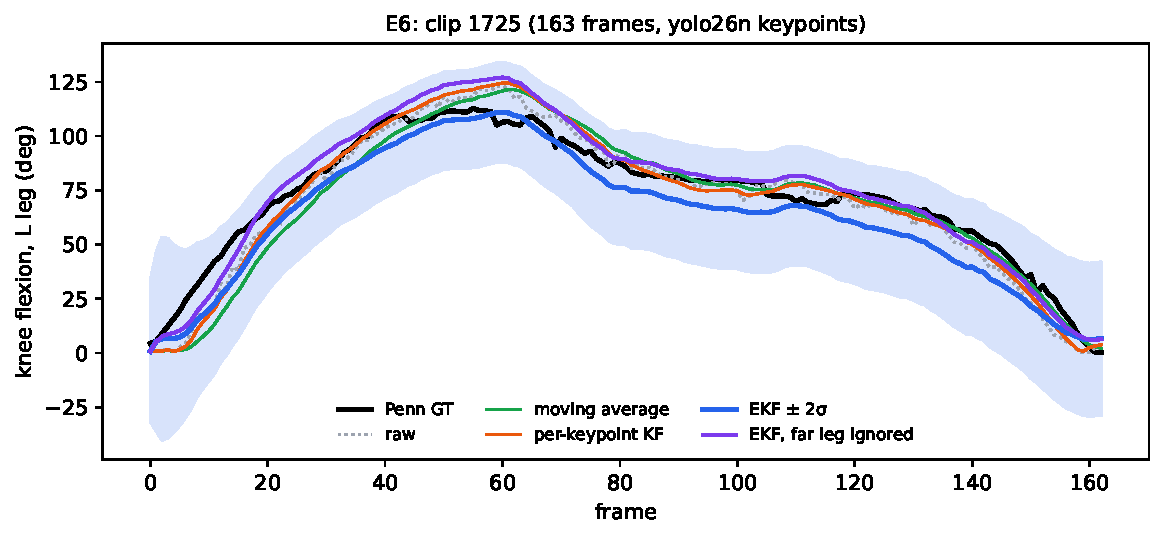
\includegraphics[width=0.9\linewidth]{e6_trace.pdf}
\caption{E6: near-side knee angle on test clip 1725 (163 frames). The EKF (blue) is smooth and its
$\pm2\sigma$ band contains the ground truth (black) throughout.}
\label{fig:e6}
\end{figure}

\paragraph{E5 (real): ablation.} Table~\ref{tab:e5real} repeats the ablation on real data. Adaptive $R$
helps on every metric (knee median $13.27\to12.86^\circ$, jitter $1.65\to1.30$, bone CV
$5.14\to4.79\%$). Gating fires on only 1.6\% of keypoints, and joint limits are never active in squats,
so both leave the medians unchanged. Re-initialisation fires 2.6 times per clip and costs a little
smoothness (jitter 1.00 without it) in exchange for the recovery shown in E4. The real NIS/dof is 0.24:
the tuned $R$ is conservative.

\begin{table}[t]
\centering\small
\caption{E5 (real, 37 test clips): EKF ablation.}
\label{tab:e5real}
\resizebox{\linewidth}{!}{%
\begin{tabular}{lccccc}
\toprule
Variant & Knee RMSE ($^\circ$) & Hip RMSE ($^\circ$) & Knee jitter & Hip jitter & Bone CV (\%)\\
\midrule
\textbf{EKF (full)}           & 12.86 & 12.08 & 1.30 & 1.56 & 4.79\\
EKF, fixed $R$                & 13.27 & 12.36 & 1.65 & 1.79 & 5.14\\
EKF, no gating                & 12.86 & 12.08 & 1.13 & 1.85 & 4.86\\
EKF, no joint limits          & 12.86 & 11.94 & 1.30 & 1.56 & 4.78\\
EKF, no re-init               & 12.86 & 12.08 & 1.00 & 1.15 & 4.89\\
EKF, fixed $R$ + no gating    & 13.27 & 12.36 & 1.47 & 1.87 & 5.27\\
\bottomrule
\end{tabular}}
\end{table}

\paragraph{E7: edge deployment.} Table~\ref{tab:e7} compares the nano and extra-large detectors with and
without the EKF. The filter adds $\approx0.5$\,ms to a 5.7\,ms detector. \textbf{YOLO26n + EKF produces
smoother angles than YOLO26x alone} (jitter 1.30 vs.\ 2.68) at about one ninth of the compute
(6.2 vs.\ 57.9\,ms/frame, i.e.\ $\approx160$ vs.\ 17 frames per second) and with more rigid bones
(CV 4.8\% vs.\ 9.0\%); YOLO26x alone remains the most accurate in angle RMSE.

\begin{table}[t]
\centering\small
\caption{E7: accuracy vs.\ runtime (RTX 2050 laptop GPU; times per frame).}
\label{tab:e7}
\resizebox{\linewidth}{!}{%
\begin{tabular}{lcccccc}
\toprule
Pipeline & Knee RMSE ($^\circ$) & Knee jitter & Bone CV (\%) & YOLO (ms) & EKF (ms) & Total (ms)\\
\midrule
YOLO26n         & 9.29  & 5.41 & 11.13 & 5.71  & --   & 5.71\\
YOLO26n + EKF   & 12.86 & 1.30 & 4.79  & 5.71  & 0.52 & 6.23\\
YOLO26x         & 8.21  & 2.68 & 9.00  & 57.91 & --   & 57.91\\
YOLO26x + EKF   & 13.45 & \textbf{0.81} & \textbf{4.56} & 57.91 & 0.51 & 58.42\\
\bottomrule
\end{tabular}}
\end{table}

\paragraph{E8: bone-length self-calibration.} Fig.~\ref{fig:e8} shows the thigh and shank length implied
by each method on clip 1725. Raw and per-keypoint-KF lengths jump by several pixels between frames; the EKF
estimates a slowly varying length with an uncertainty band. The ground-truth curve itself varies from 55 to
85\,px within the clip, because the thigh rotates towards and away from the camera (foreshortening).

\begin{figure}[t]
\centering
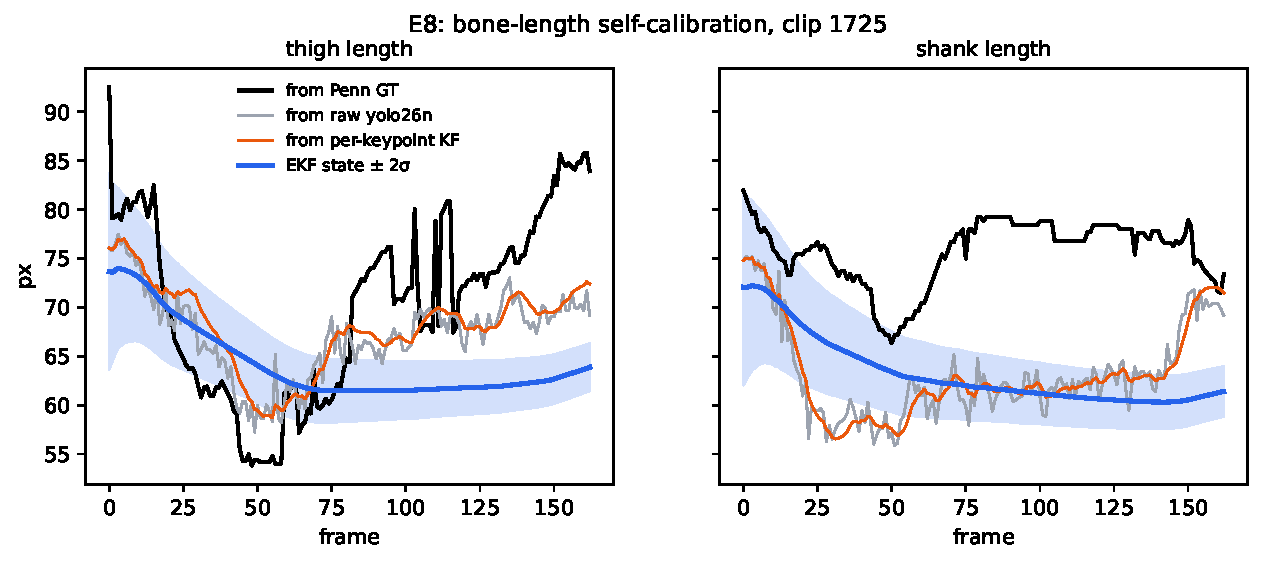
\includegraphics[width=0.9\linewidth]{e8_bone_lengths.pdf}
\caption{E8: thigh (left) and shank (right) length on clip 1725, from the ground truth, raw YOLO26n, the
per-keypoint KF, and the EKF's length state $\pm2\sigma$.}
\label{fig:e8}
\end{figure}

\paragraph{E10: qualitative result.} Fig.~\ref{fig:overlay} overlays the skeletons on four frames.

\begin{figure}[t]
\centering
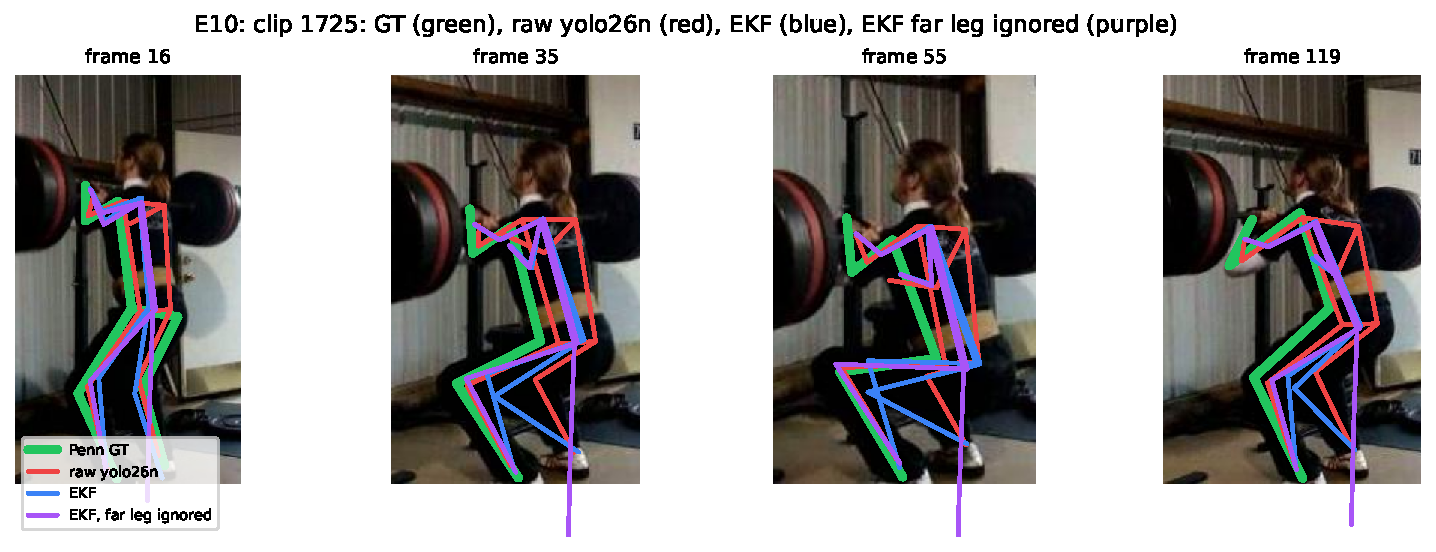
\includegraphics[width=\linewidth]{e10_overlay.pdf}
\caption{E10: clip 1725, ground truth (green), raw YOLO26n (red), EKF (blue) and EKF with the occluded leg
masked (purple). Note the raw far-side leg (frames 35, 55), which the detector reports with high
confidence although it is hidden behind the near leg.}
\label{fig:overlay}
\end{figure}

% ============================================================================ 5 DISCUSSION
\section{Discussion}
\label{sec:discussion}

\paragraph{What the EKF buys.} Across simulation and real data the EKF delivers what a per-keypoint filter
cannot: a joint angle with an uncertainty estimate, bones that keep their length (CV more than halved on
real data and below the ground truth's own 9.3\%), continuous output through dropouts, and robustness to
confident outliers (Table~\ref{tab:e5sim}). Its jitter on real data (1.30) is below that of the
hand-labelled ground truth (2.36), which itself contains annotation noise. Because the filter's cost is
only $\approx0.5$\,ms, these properties come almost for free on an edge device.

\paragraph{Process vs.\ measurement noise.} E2 shows the classic trade-off: $Q$ and $R$ decide whether the
filter believes its motion model or the detector, and the jitter and lag metrics make that trade-off
visible. On real data the tuned $\sigma_0=16$\,px is larger than YOLO's typical keypoint error: a larger
$R$ partly compensates for errors the model does not describe (wrong-side keypoints, foreshortening), so the
filter trades some responsiveness for robustness. The real NIS/dof of 0.24 confirms the tuned $R$ is
conservative.

\paragraph{Consistency.} E3 is the strongest evidence that the implementation is correct: with a matched
model the NEES and NIS are at their theoretical values. Under model mismatch (a squat is not a
constant-velocity motion) the filter errs on the safe side, reporting more uncertainty than it has, rather
than becoming overconfident.

\paragraph{Linearisation limits and creativity.} E4 showed where the EKF's local linearisation breaks: after
a long coast the uncertainty is not Gaussian in the angles and the gate wrongly rejects the true
measurement. The re-initialisation rule is a targeted, cheap fix that turns a permanent failure into a
recovery within a few frames. A UKF \cite{julier} or particle filter would represent the curved
uncertainty directly, at higher cost.

\subsection{Limitations}
\label{sec:limits}

\begin{itemize}[itemsep=3pt]
    \item \textbf{Self-occluded far leg.} In a side view the far leg is hidden behind the near leg, yet
          YOLO reports its knee and ankle with confidence typically above 0.95 (Fig.~\ref{fig:overlay}).
          Confidence-adaptive $R$ cannot reject these guesses. Because left and right share one thigh and
          one shank length, the wrong far-leg keypoints bend the shared lengths and, through them, the
          near-leg angles; this is why the plain EKF's knee RMSE ($12.86^\circ$) is above raw YOLO's
          ($9.60^\circ$) in Table~\ref{tab:e6}. Masking the far knee and ankle (side taken from the camera
          view label) restores the accuracy to $9.35^\circ$ while keeping the smoothness and rigidity.
    \item \textbf{Planar model, constant lengths.} The model is 2D. When a limb rotates out of the image
          plane its projected length changes (E8; ground truth bone CV 9.3\%), which a constant-length model
          can only follow slowly through the length random walk.
    \item \textbf{Heuristic recovery.} Re-initialisation discards the limb's history and uses a fixed
          threshold of 3 frames; it is not derived from a probabilistic model.
    \item \textbf{Scope.} Only side-view squats were evaluated, without a known frame rate ($\Delta t = 1$
          frame).
\end{itemize}

\subsection{Future work}

The far-leg problem has a direct fix that keeps the EKF at its core. First, the occluded side can be found
from the pose itself: the person's facing direction (knees ahead of ankles, wrists ahead of shoulders)
identified the camera-facing side in 47 of 47 clips, so no camera metadata is needed. Second, a fixed-lag
Rauch--Tung--Striebel smoother \cite{rts} run after the EKF refines each frame using the next few frames.
In a preliminary test, the EKF with the occluded leg masked plus a 10-frame (0.33\,s at 30\,fps) fixed-lag
smoother reached median knee and hip errors of $7.94^\circ$ and $9.72^\circ$, below raw YOLO's
$9.60^\circ$ and $10.11^\circ$, with jitter 0.68. As the lag was chosen on the test clips, these numbers are
indicative only and the lag should be tuned on the tuning set. Other directions are separate left and right
bone lengths, a 3D skeleton with a camera model, and a UKF or interacting multiple-model filter for
non-squat motions.

% ============================================================================ 6 CONCLUSION
\section{Conclusion}

This project implemented an Extended Kalman Filter that tracks a 29-state planar skeleton from monocular
YOLO26-Pose keypoints, with a nonlinear forward-kinematics measurement model, an analytic Jacobian, and four
robustness additions: confidence-adaptive $R$ with partial updates, per-keypoint $\chi^2$ gating, joint-limit
projection and track-loss re-initialisation. In simulation the filter is statistically consistent
(NEES/dim 1.03, NIS/dof 0.99), more accurate than raw keypoints and a per-keypoint Kalman filter
($5.1^\circ$ vs.\ $9.6^\circ$ and $7.0^\circ$), and recovers from long occlusions. On real Penn Action
squats it produces $4\times$ smoother joint angles, more than halves bone-length variation, keeps an
estimate in 99.9\% of frames and costs about 0.5\,ms per frame, so a nano detector with the EKF gives
smoother angles than a nine-times larger detector. The analysis identified the remaining error source,
confident detections of the hidden leg, and a concrete path to remove it.

% ============================================================================ REFERENCES
\begin{thebibliography}{99}
\small
\bibitem{kalman} R.~E. Kalman, ``A new approach to linear filtering and prediction problems,''
  \emph{Journal of Basic Engineering}, vol.~82, no.~1, pp.~35--45, 1960.
\bibitem{simon} D.~Simon, \emph{Optimal State Estimation: Kalman, $H_\infty$, and Nonlinear Approaches}.
  Wiley, 2006.
\bibitem{barshalom} Y.~Bar-Shalom, X.~R. Li, and T.~Kirubarajan, \emph{Estimation with Applications to
  Tracking and Navigation}. Wiley, 2001.
\bibitem{simon_constraints} D.~Simon, ``Kalman filtering with state constraints: a survey of linear and
  nonlinear algorithms,'' \emph{IET Control Theory \& Applications}, vol.~4, no.~8, pp.~1303--1318, 2010.
\bibitem{julier} S.~J. Julier and J.~K. Uhlmann, ``Unscented filtering and nonlinear estimation,''
  \emph{Proceedings of the IEEE}, vol.~92, no.~3, pp.~401--422, 2004.
\bibitem{rts} H.~E. Rauch, F.~Tung, and C.~T. Striebel, ``Maximum likelihood estimates of linear dynamic
  systems,'' \emph{AIAA Journal}, vol.~3, no.~8, pp.~1445--1450, 1965.
\bibitem{penn} W.~Zhang, M.~Zhu, and K.~G. Derpanis, ``From actemes to action: A strongly-supervised
  representation for detailed action understanding,'' in \emph{Proc. ICCV}, 2013.
\bibitem{coco} T.-Y. Lin \emph{et al.}, ``Microsoft COCO: Common objects in context,'' in
  \emph{Proc. ECCV}, 2014.
\bibitem{ultralytics} Ultralytics, ``Ultralytics YOLO (YOLO26 pose models),''
  \url{https://github.com/ultralytics/ultralytics}.
\bibitem{winter} D.~A. Winter, \emph{Biomechanics and Motor Control of Human Movement}, 4th~ed. Wiley, 2009.
\end{thebibliography}


\end{document}
